\chapter{Perancangan}
\label{chap:perancangan}

Pada bab ini akan dijelaskan perancangan mengenai simulator yang akan dibangun untuk pertumbuhan wirausaha. Perancangan yang dibuat akan meliputi diagram kelas beserta penjelasannya dan rancangan antarmuka dari perangkat lunak.


\section{Diagram Kelas}
\label{sec:perancangankelas}

Dalam membuat simulator diperlukan sebuah GUI atau Interface untuk bisa menggambarkan kinerja suatu sistem. Berdasarkan hasil pengembangan diagram kelas pada bab analisis \ref{fig:CD1}, dibuatlah diagram kelas rinci untuk memenuhi kebutuhan dalam membangun simulator. Deskripsi kelas beserta fungsinya akan dijelaskan pada subbab selanjutnya. (Gambar \ref{fig:classdiagram2})

\begin{figure} [H]
	\centering  
	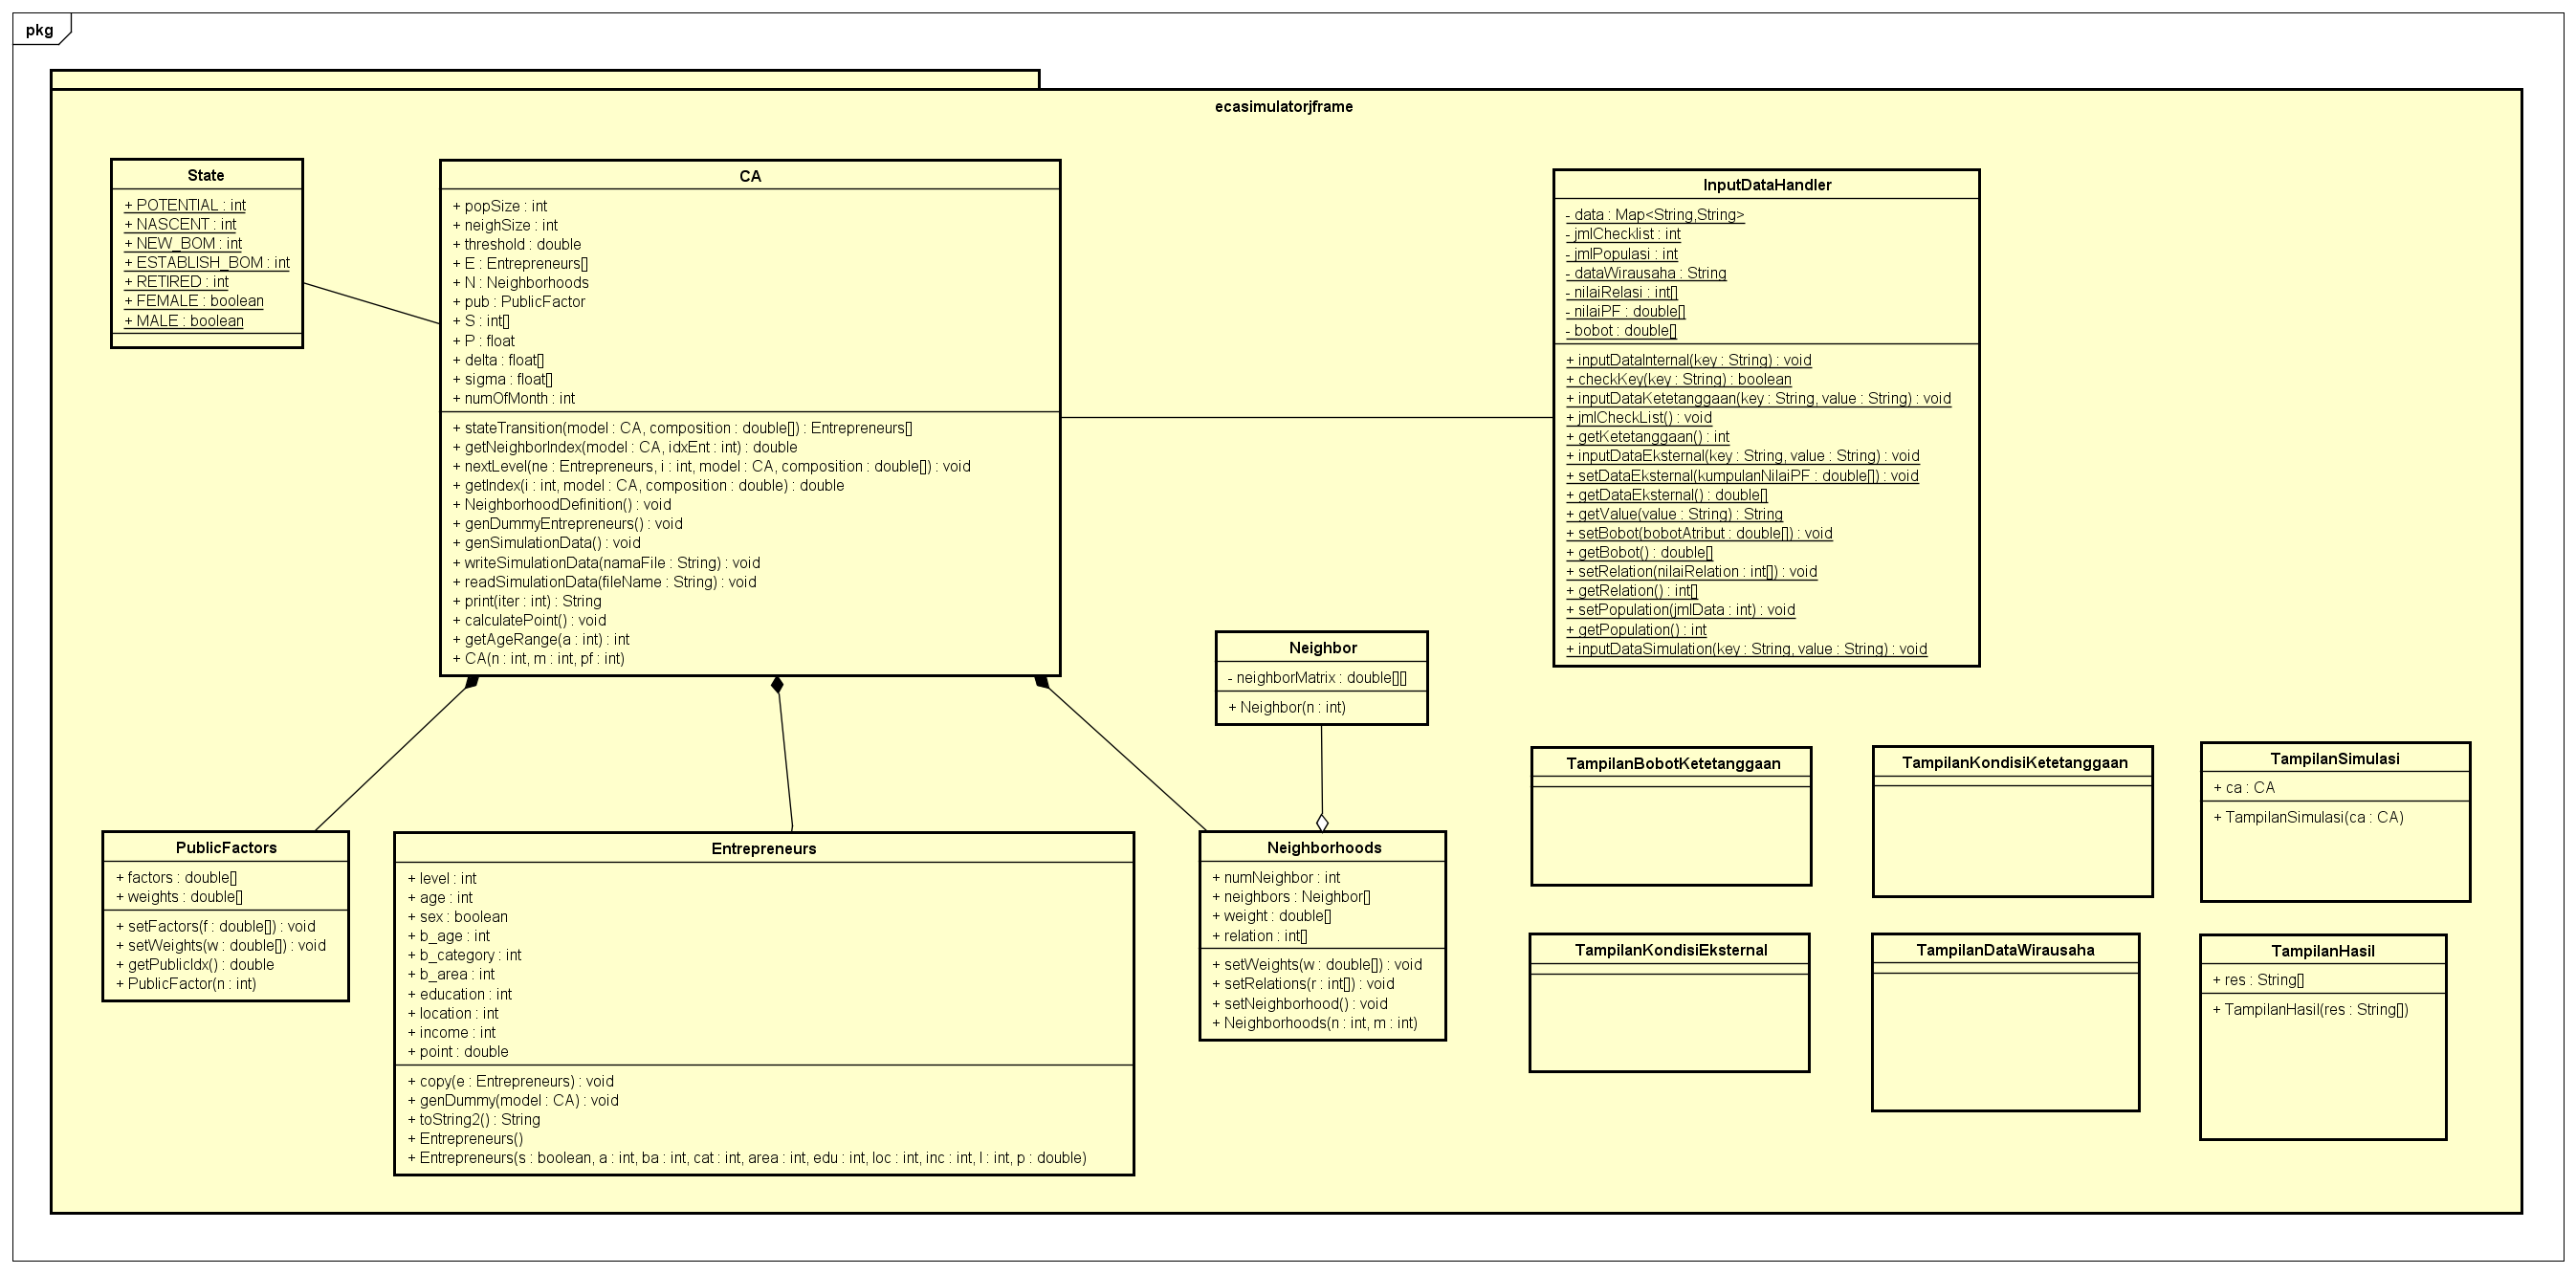
\includegraphics[width=16cm, height=25cm]{diagramKelas1}
	\caption[Diagram Kelas Simulator ECA]{Diagram Kelas Simulator ECA} 
	\label{fig:classdiagram2} 
\end{figure}

\subsection{Kelas CA}
Dilakukan perubahan pada tiga method di kelas CA yaitu :
\begin{itemize}
	\item \texttt{public Entrepreneur[] stateTransition(CA model, double[] composition)}\\
	Perubahan yang dilakukan adalah pada saat menambahkan umur wirausaha. Umur wirausaha akan ditambah jika bulannya sudah mencapai 12 bulan atau kelipatan 12 bulan. Dilakukan perubahan agar pada setiap iterasi (bulan), umur wirausaha tidak bertambah secara terus-menerus melainkan ditambah pada saat sudah 1 tahun (12 bulan).
	\item \texttt{public void NeighborhoodDefinition() }\\
	Perubahan yang dilakukan adalah penambahan pada faktor (umur, pendidikan, pendapatan dan jenis kelamin) dan relasi (lebih dari sama dengan).
	\item \texttt{public void calculatePoint(double[] POAm, double[] POAf, double[] POEf, double[] POEm, double[] POLm, double[] POLf, double[] POIm, double[] POIf, double[] PCAf, double[] PCAm, double[] PCEm, double[] PCEf, double[] PCLm, double[] PCLf, double[] PCIm, double[] PCIf, double[] RMAm, double[] RMAf, double[] RMIm, double[] RMIf, double[] FFAf, double[] FFAm, double[] FFEf, double[] FFEm, double[] FFLf, double[] FFLm, double[] MALf, double[] MALm, double[] MAIf, double[] MAIm, double[] HSSIf, double[] HSSIm, double[] HSSLf, double[] HSSLm, double[] HSSAf, double[] HSSAm, double[] HSSEf, double[] HSSEm)}\\
	Perubahan yang dilakukan adalah penambahan pada indikator yang mendukung intensi masyarakat untuk memulai usaha. Indikator-indikator tersebut yaitu Entrepreneurial Intentions (High Status Successful Entrepreneurship, Media Attention) dan Fear of Failure.
\end{itemize}



\subsection{Kelas TampilanBobotKetetanggaan}
Kelas ini merupakan kelas untuk menampilkan seluruh atribut umum dari seorang wirausaha yang dapat dipilih menggunakan \textit{checkbox}, atribut yang dipilih nantinya akan mempengaruhi ketetanggaan antara wirausaha yang satu dengan wirausaha lainnya. Setelah itu, \textit{user} diminta mengisi bobot untuk masing-masing atribut yang sudah dichecklist melalui \textit{textfield}.

\subsection{Kelas TampilanKondisiKetetanggaan}
Kelas ini merupakan kelas untuk menampilkan atribut yang sudah dipilih dari kelas TampilanKondisiInternal. \textit{User} dapat memilih atribut mana saja yang akan ditetapkan menjadi kondisi ketetanggaan untuk satu wirausaha ke wirausaha lainnya. Selain itu, \textit{user} diminta untuk mengisi hubungan ketetanggaan khusus untuk 4 atribut yaitu umur, level, pendapatan dan pendidikan jika \textit{user} men-checklist salah satu atau bahkan keempat-empatnya dari atribut tersebut. Untuk atribut jenis kelamin, lokasi usaha dan bidang usaha tidak dapat ditetapkan menjadi 3 jenis karena jenisnya hanya satu yaitu sama dengan. Alasan ketiga atribut tersebut tidak bisa ditetapkan menjadi 3 jenis karena ketiga atribut tersebut tidak bisa diurutkan atau dibandingkan seperti atribut a lebih besar dari atribut b.

\subsection{Kelas TampilanKondisiEksternal}
Kelas ini merupakan kelas untuk menampilkan faktor eksternal yang mempengaruhi pertumbuhan wirausaha. Dalam kasus ini ditetapkan 4 faktor saja yaitu program pemerintah, dinamika pasar, norma,sosial dan budaya, serta infrastruktur fisik dan akses layanan. \textit{User} diminta untuk mengisi bobot untuk setiap faktor dan total dari semua bobot harus 100\%.

\subsection{Kelas DataWirausaha}
Kelas ini merupakan kelas untuk membuka file data wirausaha yang akan disimulasikan, lalu menampilkannya ke tabel. Isi datanya berupa :
\begin{enumerate}
	\item Jenis Kelamin
	\item Umur
	\item Usia Bisnis
	\item Kategori Usaha
	\item Subkategori
	\item Pendidikan
	\item Lokasi
	\item Pendapatan
	\item Level
	\item Point
\end{enumerate}

\subsection{Kelas TampilanSimulasi}
Kelas ini berfungsi untuk mengisi nilai a, b, c, threshold dan periode. Nilai a,b,c dan threshold bertipe double, sedangkan periode bertipe integer. Periode ini dihitung dalam bulan. Kelas ini juga untuk menghitung Continuity Index yang hasil iterasinya akan dikirim ke kelas TampilanHasil dalam bentuk tabel. Selain itu, kelas ini juga akan menampilkan hasil perubahan setiap individu wirausaha dalam setiap bulannya pada file CSV.

\subsection{Kelas TampilanHasil}
Kelas ini berfungsi untuk menampilkan iterasi (per bulan) banyaknya wirausaha yang berada pada level tertentu dalam bentuk tabel.

\subsection{Kelas InputDataHandler}
Kelas ini merupakan kelas untuk mengambil dan menyimpan data masukan dari \textit{user} yang nantinya akan dipakai untuk menghitung Continuity Index.
Berikut penjelasan method-method yang ada di kelas InputDataHandler :
	\begin{itemize}
		\item \texttt{public static void inputDataInternal(String key, String value)}\\
		Berfungsi untuk menyimpan masukan pada kelas TampilanBobotKetetanggaan.\\
		Parameter :
		\begin{itemize}
			\item \texttt{key} merupakan kata kunci dari setiap masukan.
			\item \texttt{value} merupakan nilai dari kata kunci.
		\end{itemize}
		
		\item \texttt{public static boolean checkKey(String key)}\\
		Berfungsi untuk memeriksa isi nilai dari kata kunci. Return \textit{true} jika kata kunci tersebut mempunyai nilai. Return \textit{false} jika kata kunci tersebut tidak mempunyai nilai.\\
		Parameter :
		\begin{itemize}
			\item \texttt{key} merupakan kata kunci dari setiap masukan.
		\end{itemize}
		
		\item \texttt{public static void inputDataKetetanggaan(String key, String value)}\\
		Berfungsi untuk menyimpan masukan pada kelas TampilanKondisiKetetanggaan.\\
		Parameter :
		\begin{itemize}
			\item \texttt{key} merupakan kata kunci dari setiap masukan.
			\item \texttt{value} merupakan nilai dari kata kunci.
		\end{itemize}
		
		\item \texttt{public static void jmlCheckList()}\\
		Berfungsi untuk menambahkan jumlah \textit{checklist} pada kelas TampilanBobotKetetanggaan.
		
		\item \texttt{public static int getKetetanggaan()}\\
		Berfungsi untuk mengambil nilai ketetanggaan.
		
		\item \texttt{public static void inputDataEksternal(String key, String value)}\\
		Berfungsi untuk menyimpan masukan dari kelas TampilanKondisiEksternal.\\
		Parameter:
		\begin{itemize}
			\item \texttt{key} merupakan kata kunci dari setiap masukan.
			\item \texttt{value} merupakan nilai dari kata kunci.
		\end{itemize}
		
		\item \texttt{public static void setDataEksternal(double[] kumpulanNilaiPF)}\\
		Berfungsi untuk mengubah nilai-nilai dari faktor publik.\\
		Parameter:
		\begin{itemize}
			\item \texttt{kumpulanNilaiPF} merupakan kumpulan nilai faktor publik.
		\end{itemize}
		
		\item \texttt{public static double[] getDataEksternal()}\\
		Berfungsi untuk mengambil nilai-nilai dari faktor publik.
		
		\item \texttt{public static String getValue(String key)}\\
		Berfungsi untuk mengambil nilai dari kata kunci.\\
		Parameter:
		\begin{itemize}
			\item \texttt{key} merupakan kata kunci dari setiap masukan.
		\end{itemize}
		
		\item \texttt{public static void setBobot(double[] bobotAtribut)}\\
		Berfungsi untuk mengubah nilai-nilai bobot dari setiap atribut.\\
		Parameter:
		\begin{itemize}
			\item \texttt{bobotAtribut} merupakan kumpulan bobot dari setiap atribut.
		\end{itemize}
		
		\item \texttt{public static void getBobot()}\\
		Berfungsi untuk mengambil nilai dari bobot.
		
		\item \texttt{public static void setRelation(int[] nilaiRelation)}\\
		Berfungsi untuk mengubah nilai-nilai dari setiap relasi.\\
		Parameter:
		\begin{itemize}
			\item \texttt{nilaiRelation} merupakan kumpulan nilai dari setiap relasi.
		\end{itemize}
		
		\item \texttt{public static int[] getRelation()}\\
		Berfungsi untuk mengambil nilai dari setiap relasi.
		
		\item \texttt{public static void setPopulation(int jmlData)}\\
		Berfungsi untuk mengubah nilai dari populasi.\\
		Parameter:
		\begin{itemize}
			\item \texttt{jmlData} merupakan jumlah dari data masukan \textit{user}.
		\end{itemize}
		
		\item \texttt{public static int getPopulation()}\\
		Berfungsi untuk mengembalikan nilai dari populasi.
		
		\item \texttt{public static void inputDataSimulasi(String key, String value)}\\
		Berfungsi untuk menyimpan masukan dari kelas TampilanSimulasi.\\
		Parameter :
		\begin{itemize}
			\item \texttt{key} merupakan kata kunci dari setiap masukan.
			\item \texttt{value} merupakan nilai dari kata kunci.
		\end{itemize}
	\end{itemize}


\section{Rancangan Antarmuka}
\label{sec:rancanganantarmuka}

\subsection{TampilanKondisiInternal}

\begin{figure} [H]
	\centering  
	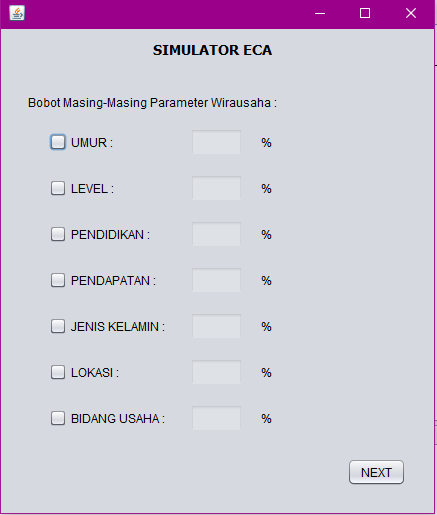
\includegraphics[width=11cm, height=12cm]{tampilanKondisiInternal} 
	\label{fig:kondisiInternal} 
\end{figure}

Dapat dilihat pada gambar \ref{fig:kondisiInternal}, pada kondisi awal terdapat 7 atribut umum dari seorang wirausahawan yang dapat dipilih oleh \textit{user} melalui \textit{checkbox}. Jika \textit{user} tidak mengisi \textit{checkbox} terlebih dahulu, \textit{user} tidak akan bisa mengisi bobot atribut. Atribut yang dipilih melalui \textit{checkbox}, akan menjadi ketetanggaan dari wirausaha satu dengan wirausaha lainnya. Setelah \textit{user} memilih atribut wirausaha, \textit{user} harus mengisi bobot dari masing-masing atribut melalui \textit{text field}. Total dari bobot atribut yang dipilih jumlahnya harus 100\%. Jika \textit{user} tidak mengisi seluruh  \textit{checkbox}, \textit{user} tidak akan bisa melanjutkan ke proses selanjutnya. Begitu juga jika \textit{user} tidak mengisi bobot berdasarkan atribut yang sudah dipilih, \textit{user} tidak dapat melanjutkan ke proses selanjutnya.

\subsection{TampilanKondisiKetetanggaan}

\begin{figure} [H]
	\centering  
	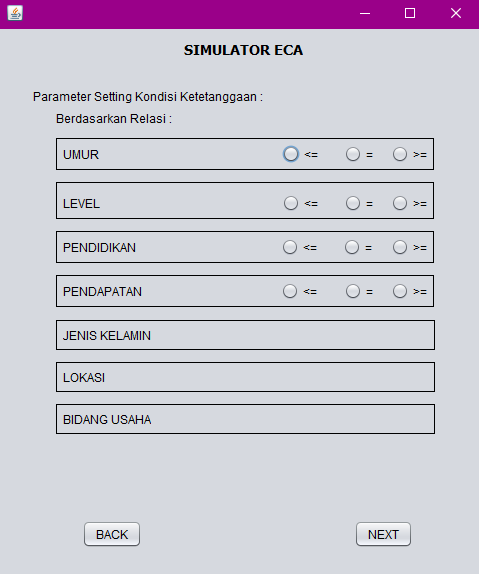
\includegraphics[width=11cm, height=12cm]{tampilanKondisiKetetanggaan} 
	\label{fig:kondisiTetangga} 
\end{figure}

Dapat dilihat pada gambar \ref{fig:kondisiTetangga}, terdapat 7 atribut tetangga yang telah dipilih oleh \textit{user} pada kelas TampilanBobotKetetanggaan. Pada tampilan ini \textit{user} diminta untuk mengisi relasi ketetanggaan khususnya pada atribut umur, level, pendapatan dan pendidikan. 3 atribut lainnya tidak terdapat relasi ketetanggaan, hal ini dikarenakan ketiga atribut tersebut tidak bisa dibanding-bandingkan. Contohnya seperti lokasi, wirausaha A membangun usahanya di kota Jakarta, sedangkan wirausaha B membangun usahanya di kota Bandung. Tentu saja hal ini tidak dapat ditetapkan sebagai kota Jakarta lebih dari kota Bandung atau kota Bandung kurang dari kota Jakarta.

\subsection{TampilanKondisiEksternal}

\begin{figure} [H]
	\centering  
	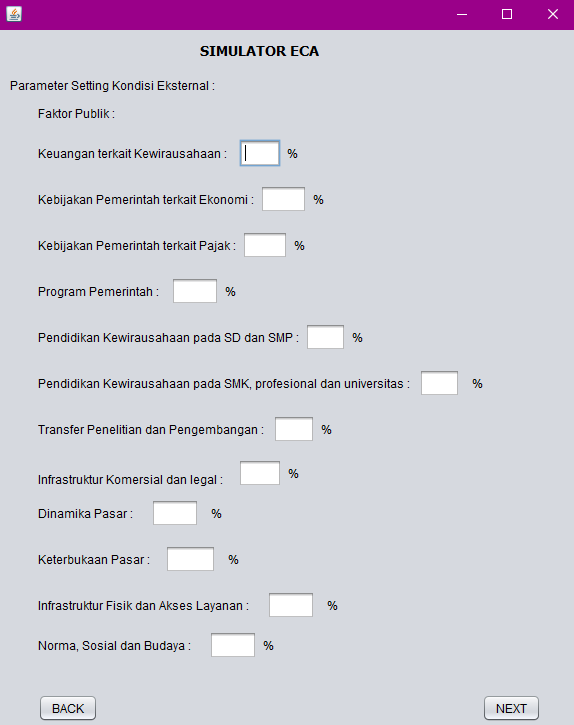
\includegraphics[width=11cm, height=13cm]{tampilanKondisiEksternal} 
	\label{fig:kondisiEksternal} 
\end{figure}

Pada tampilan kondisi eksternal terdapat 12 faktor publik berdasarkan GEM 2013. Untuk keduabelas faktor ini, \textit{user} harus mengisi bobot setiap faktor publik yang total bobotnya harus 100\%. 

\subsection{TampilanDataWirausaha}

\begin{figure} [H]
	\centering  
	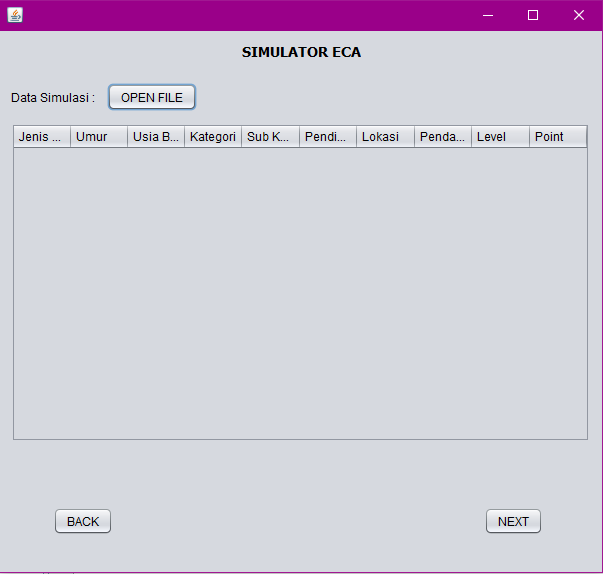
\includegraphics[width=13cm, height=12cm]{tampilanDataWirausaha1} 
	\label{fig:kondisiDataWirausaha} 
\end{figure}

Tampilan ini berfungsi untuk memasukkan file data wirausaha dalam format text.


\begin{figure} [H]
	\centering  
	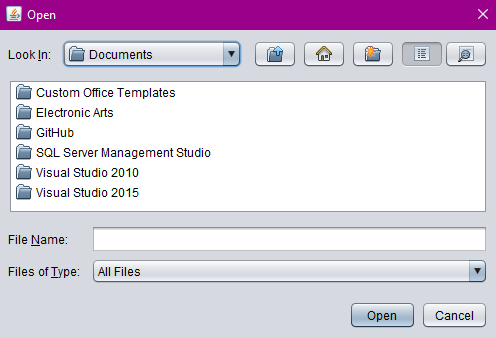
\includegraphics[width=11cm, height=9cm]{tampilanBukaFile} 
	\label{fig:bukaFile} 
\end{figure}



\subsection{TampilanSimulasi}

\begin{figure} [H]
	\centering  
	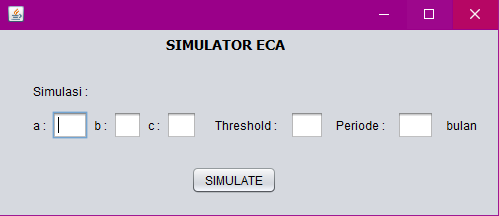
\includegraphics[width=11cm, height=7cm]{tampilanSimulasii} 
	\label{fig:simulasi} 
\end{figure}

Pada tampilan simulasi, \textit{user} diminta untuk mengisi nilai a,b,c, threshold dan periode. Total dari nilai a,b dan c harus 1. Periode merupakan berapa lama iterasi tersebut akan berjalan (dalam bulan). Sedangkan \textit{button} "SIMULATE" berfungsi untuk menjalankan simulasi yang hasilnya akan ditampilkan dalam bentuk tabel.

\subsection{TampilanHasil}

\begin{figure} [H]
	\centering  
	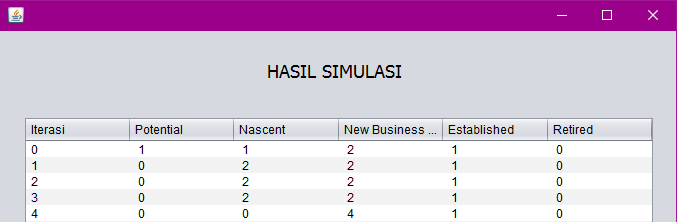
\includegraphics[width=11cm, height=7cm]{tampilanHasil1} 
	\label{fig:tampilanHasil} 
\end{figure}

